\section{Preprocessing - Spliting Data}

Ο κώδικας ξεκινάει με την εισαγωγή των κατάλληλων βιβλιοθηκών συγκεκριμένα την
sklearn, pandas, matplotlib, os, numpy . Στην συνέχεια μέσω της pandas διαβάζεται
το dataset το οποίο είναι χωρισμένο σε 4 τύπου csv αρχεία. Μέσω της εντολής \textbf{pd.concat}
δημιουργήθηκε ένα κοινό αρχείο, το οποίο με την εντολή info ελεγχθηκε εάν ήταν
επιτυχής η ένωση των 4 τύπου csv , όπως και το μέγεθος του πίνακα. Με την εντολή
\textbf{data.isnull().sum().head} ελέχθηκε εάν λείπουν δεδομένα, και με την εντολή \textbf{order = data[64].unique()} τυπώθηκε ο αριθμός των κλάσεων οι οποίες βρίσκονται στην στήλη 64, και με την εντολή \stextbf{data[64].value counts().sort values(ascending=False)} τυπώθηκε το μέγεθΔιάγραμμαος της κάθε κλάσης. Εφόσον όλα ήταν καλά, χωρίστηκε η βάση σε δύο παραμέτρους/λίστες X, y. Η λίστα X περιέχει όλες τις λίστες πλήν της στήλης
"label". Από την άλλη η λίστα y περιέχει μόνο την στήλη "label". Μετά τον διαχωρισμό
της βάσης σε δύο λίστες. Μετά τον διαχωρισμό της βάσης σε δύο λίστες, ορίστηκαν
τέσσερις παράμετροι με βάση τις δύο λίστες με την εντολή X train, X test, y train, y
test = train test split(X, y, random state=40).
Στην συνέχεια χρησιμοποιήθηκε η εντολή \textbf{StandardScaler} στις λίστες Χ train, X test, η οποία τυποποιεί  τα χαρακτηριστικά αφαιρώντας τη μέση τιμή και κλιμακώνοντας τη διακύμανση, ώστε να είναι πιο έυκολο να χρησιμοποιηθούν αργότερα από τα μοντέλα.

\section{KPCA}

Στην συνέχεια εισάχθηκαν οι κατάλληλες εντολές μέσω της sklearn για να εφαρμοστεί η \textbf{KPCA} με δύο διαφορετικούς Κernels (RBF, Sigmoid) στις λίστες Χ train και Χ test (μετά την τυποποίηση τους).

\subsection{KPCA with RBF Kernel}

\subsubsection{Visualization and building of KPCA}
Αρχικά έπρεπε να βρεθεί ο αριθμός των components που θα κρατηθούν ώστε να έχουμε το $91\%$ της πληροφορίας του. Αυτό επιτεύχθηκε με την βοήθεια του διαγράμματος \ref{f:g5}, στο οποίο φαίνεται πόσα components πρέπει να βάλουμε στον αλγόριθμο του \textbf{KPCA} ώστε να κρατήσουμε την πληροφορία που ζητάμε. Έτσι μέσω αυτού του διαγράμματος και με την επαλήθευση του με την βοήθεια της εντολής \textbf{loc} της βιβλιοθήκης pandas βρέθηκε το πλήθος των χαρακτηριστικών που πρέπει να κρατηθούν , που είναι 44.

\begin{figure}[ht]
	\centering
	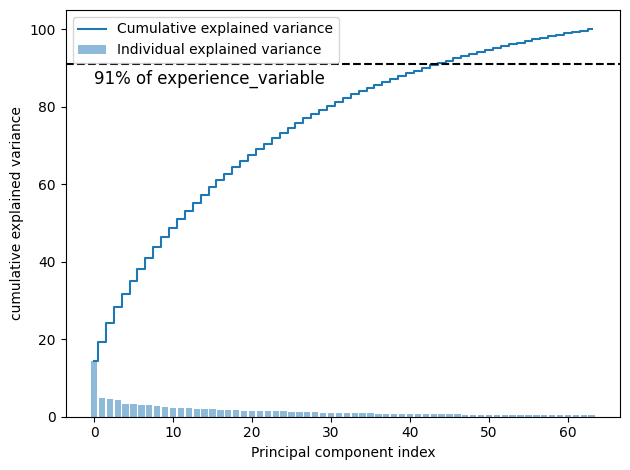
\includegraphics[width=1\linewidth]{Images data1/KPCARBF2plot.png}
	\caption{ Διάγραμμα Cumulative Variance - Principal Components }
	\label{f:g5}	
\end{figure}
\clearpage
\subsubsection{Training SVM KNN NCC Models}

\paragraph{Linear Model}

Αναπτύχθηκε το πρώτο μοντέλο, το οποίο είναι το γραμμικό SVM, και
τυπώθηκε το ποσοστό ακρίβειας στο training και στο testing του μοντέλου. To train accuracy είναι 0.44 ενώ το test
accuracy είναι 0.438. Ο χρόνος εκπαίδευσης του μοντέλου ήταν περίπου 5.1 seconds.

\paragraph{RBF Model}
\clearline
Το δεύτερο μοντέλο που υλοποιήθηκε ήταν το RBF SVM. Και εδώ τυπώθηκαν τα ποσοστά
ακρίβειας στο training και στο testing του μοντέλου. To train accuracy είναι 0.9462 ενώ το test accuracy είναι 0.887. Ο χρόνος εκπαίδευσης του μοντέλου ήταν περίπου 7.4 seconds.
Έπειτα χρησιμοποιήθηκε η εντολή \textbf{GridSearchCV} με την οποία έγινε cross-validation για συγκεκριμένες παραμέτρους C : [4, 6, 10, 20, 25] και gamma : [′scale', 0.01, 0.1, 0.0001]. Τυπώθηκαν τα αποτελέσματα του καλύτερου
συνδυασμού παραμέτρων για τον πυρήνα RBF οι οποίες είναι gamma : [′scale′] και C :
[4] με ποσοστό ακρίβειας στο train και test 0.99, 0.889.

\paragraph{KNN Model}
Ακολούθως εκπαιδεύτηκε το τρίτο μοντέλο στα δεδομένα, με το train accuracy να φτάνει 0.86, ενώ το test accuracy να πέφτει στο 0.75. Ο χρόνος εκπαίδευσης είναι 0.4 seconds.
\paragraph{NCC}
Τέλος πραγματοποιήθηκε η εκπαίδευση για το NCC μοντέλο, του οποίου το train accuracy είναι 0.5 , και το test accuracy είναι 0.495. Ο χρόνος εκπαίδευσης είναι 0.1 seconds.
\subsection{KPCA+LDA with RBF Kernel}

Το επόμενο βήμα στην εργασία ήταν να υλοποιηθεί ο αλγόριθμος LDA πάνω στις λίστες που παρήχθησαν μέσω του \textbf{KPCA}
\subsubsection{Searching the best component  and building LDA  }

Στην αρχή όπως και στον \textbf{KPCA}, μέσω του κώδικα, επιλέχθηκε το πλήθος των component που χρειάζονται ώστε να κρατηθεί το ίδιο ποσοστό πληροφορίας με πριν ($91\%$), ώστε στην συνέχεια να εφαρμοστεί στον αλγόριθμο, το οποίο στην συγκεκριμένη περίπτωση ήταν \emph{1}.

\subsubsection{Training SVM KNN NCC Models}

\paragraph{Linear Model}

Αναπτύχθηκε το πρώτο μοντέλο, το οποίο είναι το γραμμικό SVM, και
τυπώθηκε το ποσοστό ακρίβειας στο training και στο testing του μοντέλου. To train accuracy είναι 0.43 ενώ το test accuracy είναι 0.445. Ο χρόνος εκπαίδευσης του μοντέλου ήταν περίπου 2.7 seconds.

\paragraph{RBF Model}

Το δεύτερο μοντέλο που υλοποιήθηκε ήταν το RBF SVM. Και εδώ τυπώθηκαν τα ποσοστά
ακρίβειας στο training και στο testing του μοντέλου. To train accuracy είναι 0.386 ενώ το test accuracy είναι 0.362. Ο χρόνος εκπαίδευσης του μοντέλου ήταν περίπου 7.7 seconds.
Έπειτα χρησιμοποιήθηκε η εντολή \textbf{GridSearchCV} με την οποία έγινε cross-validation για συγκεκριμένες παραμέτρους C : [4, 6, 10, 20, 25] και gamma : [′scale', 0.01, 0.1, 0.0001].Τυπώθηκαν τα αποτελέσματα του καλύτερου
συνδυασμού παραμέτρων για τον πυρήνα RBF οι οποίες είναι gamma : [′scale′] και C :
[20] με ποσοστό ακρίβειας στο train και test 0.44, 0.46.

\paragraph{KNN Model}
Ακολούθως εκπαιδεύτηκε το τρίτο μοντέλο στα δεδομένα, με το train accuracy να φτάνει 0.689, ενώ το test accuracy να πέφτει στο 0.385. Ο χρόνος εκπαίδευσης είναι 0.3 seconds
\paragraph{NCC}
Τέλος πραγματοποιήθηκε η εκπαίδευση για το NCC μοντέλο, του οποίου το train accuracy είναι 0.42, και το test accuracy είναι 0.44. Ο χρόνος εκπαίδευσης είναι 0.1 seconds.
\clearpage


\subsection{KPCA with Sigmoid Kernel}
\subsubsection{Visualization and building of KPCA}
Αρχικά έπρεπε να βρεθεί ο αριθμός των components που θα κρατηθούν ώστε να έχουμε το $91\%$ της πληροφορίας του. Αυτό επιτεύχθηκε με την βοήθεια του διαγράμματος \ref{f:g6}, στο οποίο φαίνεται πόσα components πρέπει να βάλουμε στον αλγόριθμο του \textbf{KPCA} ώστε να κρατήσουμε την πληροφορία που ζητάμε. Έτσι μέσω αυτού του διαγράμματος και με την επαλήθευση του με την βοήθεια της εντολής \textbf{loc} της βιβλιοθήκης pandas βρέθηκε το πλήθος των χαρακτηριστικών που πρέπει να κρατηθούν , που είναι 44.

\begin{figure}[ht]
	\centering
	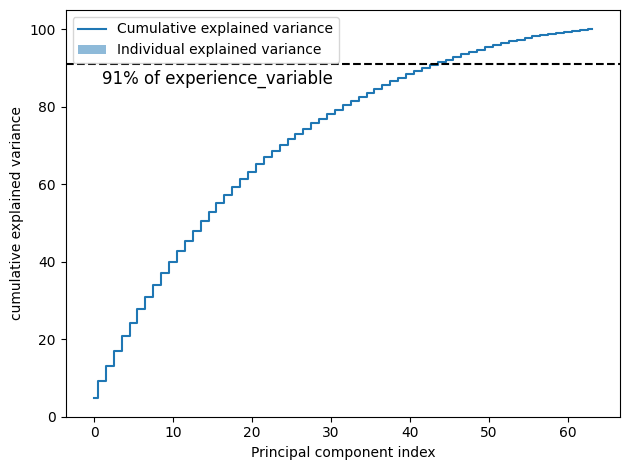
\includegraphics[width=1\linewidth]{Images data1/KPCAsigm2plot.png}
	\caption{ Διάγραμμα Cumulative Variance - Principal Components   }
	\label{f:g6}	
\end{figure}
\clearpage
\subsubsection{Training SVM KNN NCC Models}

\paragraph{Linear Model}

Αναπτύχθηκε το πρώτο μοντέλο, το οποίο είναι το γραμμικό SVM, και
τυπώθηκε το ποσοστό ακρίβειας στο training και στο testing του μοντέλου. To train accuracy είναι 0.3 ενώ το test
accuracy είναι 0.27. Ο χρόνος εκπαίδευσης του μοντέλου ήταν περίπου 6.1 seconds.

\paragraph{RBF Model}
\clearline
Το δεύτερο μοντέλο που υλοποιήθηκε ήταν το RBF SVM. Και εδώ τυπώθηκαν τα ποσοστά
ακρίβειας στο training και στο testing του μοντέλου. To train accuracy είναι 0.935 ενώ το test accuracy είναι 0.89. Ο χρόνος εκπαίδευσης του μοντέλου ήταν περίπου 7.2 seconds.
Έπειτα χρησιμοποιήθηκε η εντολή \textbf{GridSearchCV} με την οποία έγινε cross-validation για συγκεκριμένες παραμέτρους C : [4, 6, 10, 20, 25] και gamma : [′scale', 0.01, 0.1, 0.0001]. Τυπώθηκαν τα αποτελέσματα του καλύτερου
συνδυασμού παραμέτρων για τον πυρήνα RBF οι οποίες είναι gamma : [′scale′] και C :
[6] με ποσοστό ακρίβειας στο train και test 0.98, 0.91.

\paragraph{KNN Model}
Ακολούθως εκπαιδεύτηκε το τρίτο μοντέλο στα δεδομένα, με το train accuracy να φτάνει 0.86, ενώ το test accuracy να πέφτει στο 0.648. Ο χρόνος εκπαίδευσης είναι 0.4 seconds.
\paragraph{NCC}
Τέλος πραγματοποιήθηκε η εκπαίδευση για το NCC μοντέλο, του οποίου το train accuracy είναι 0.2959 , και το test accuracy είναι 0.266. Ο χρόνος εκπαίδευσης είναι 0.1 seconds.
\subsection{KPCA+LDA with Sigmoid Kernel}

Το επόμενο βήμα στην εργασία ήταν να υλοποιηθεί ο αλγόριθμος LDA πάνω στις λίστες που παρήχθησαν μέσω του \textbf{KPCA}
\subsubsection{Searching the best component  and building LDA  }

Στην αρχή όπως και στον \textbf{KPCA}, μέσω του κώδικα, επιλέχθηκε το πλήθος των component που χρειάζονται ώστε να κρατηθεί το ίδιο ποσοστό πληροφορίας με πριν ($91\%$), ώστε στην συνέχεια να εφαρμοστεί στον αλγόριθμο, το οποίο στην συγκεκριμένη περίπτωση ήταν \emph{3}.

\subsubsection{Training SVM KNN NCC Models}

\paragraph{Linear Model}

Αναπτύχθηκε το πρώτο μοντέλο, το οποίο είναι το γραμμικό SVM, και
τυπώθηκε το ποσοστό ακρίβειας στο training και στο testing του μοντέλου. To train accuracy είναι 0.31 ενώ το test accuracy είναι 0.278. Ο χρόνος εκπαίδευσης του μοντέλου ήταν περίπου 3.3 seconds.

\paragraph{RBF Model}

Το δεύτερο μοντέλο που υλοποιήθηκε ήταν το RBF SVM. Και εδώ τυπώθηκαν τα ποσοστά
ακρίβειας στο training και στο testing του μοντέλου. To train accuracy είναι 0.386 ενώ το test accuracy είναι 0.362. Ο χρόνος εκπαίδευσης του μοντέλου ήταν περίπου 7.6 seconds.
Έπειτα χρησιμοποιήθηκε η εντολή \textbf{GridSearchCV} με την οποία έγινε cross-validation για συγκεκριμένες παραμέτρους C : [4, 6, 10, 20, 25] και gamma : [′scale', 0.01, 0.1, 0.0001].Τυπώθηκαν τα αποτελέσματα του καλύτερου
συνδυασμού παραμέτρων για τον πυρήνα RBF οι οποίες είναι gamma : [0.1] και C :
[4] με ποσοστό ακρίβειας στο train και test 0.37, 0.367.

\paragraph{KNN Model}
Ακολούθως εκπαιδεύτηκε το τρίτο μοντέλο στα δεδομένα, με το train accuracy να φτάνει 0.649, ενώ το test accuracy να πέφτει στο 0.289. Ο χρόνος εκπαίδευσης είναι 0.3 seconds
\paragraph{NCC}
Τέλος πραγματοποιήθηκε η εκπαίδευση για το NCC μοντέλο, του οποίου το train accuracy είναι 0.3 , και το test accuracy είναι 0.268. Ο χρόνος εκπαίδευσης είναι 0.1 seconds.
\clearpage
\section{Σύγκριση μοντέλων}
Στην παράγραφο αυτήν θα συγκριθούν τα μοντέλα που προέκυψαν ύστερα από την εφαρμογή των αλγορίθμων KPCA και LDA, με τα μοντέλα της 1ης εργασίας.

\subsection{RBF Kernel}
Αρχικά θα συγκριθούν τα μοντέλα της KPCA+LDA με RBF Kernel, με της 1ης εργασίας
\subsubsection{Original Linear SVM vs KPCA+LDA Linear SVM}
Στα γραμμικά μοντέλα παρατηρείται ότι μετά το \textbf{KPCA +LDA}, το train accuracy ανεβαίνει απο 0.39 στην 1η εργασία σε 0.433. Το ίδιο συμβαίνει και στο test accuracy που απο 0.34 στην 1η εργασία φτάνει το 0.445.Επίσης παρατηρείται μείωση του χρόνο εκτέλεσης απο 12.9 seconds σε 2.7 seconds.
\subsubsection{Original RBF SVM vs KPCA+LDA RBF SVM}
Απο την άλλη στα RBF μοντέλα των KPCA+LDA. τόσο το train όσο και το test accuracy πέφτουν κατα 0.5 ακόμα και μετά το cross-validation. Συγκεκριμένα το αρχικό RBF μοντέλο έχει 0.926 test accuracy ενώ το KPCA+LDA μοντέλο έχει 0.46. Επίσης ο χρόνος εκτέλεσης ανεβαίνει κατα 4 second στo KPCA+LDA RBF μοντέλο, απο 4.6 seconds σε 8.7.
\subsubsection{Original KNN vs KPCA+LDA KNN}
Στο συγκεκριμένο μοντέλο παρατηρείται οτι το train accuracy για το KPCA+LDA είναι μικρότερο κατα 0.1, στο 0.689 και το test accuracy είναι μειωμένο κατα σχεδόν 0.3 στο 0.385, απο 0.66.
Ο χρόνος εκπαίδευσης και των δύο KNN είναι σχεδόν ίδιος.
\subsubsection{Original NCC vs KPCA+LDA NCC}
Τέλος τo test, train accuracy tou KPCA+LDA NCC μοντέλου είναι 0.42 και 0.44 αντίστοιχα. Δηλαδή παρατηρείται αύξηση στο συγκεκριμένο μοντέλο έναντι των αρχικού test, train accuracy
(0.33, 0.296 αντίστοιχα). Ο χρόνος εκπαίδευσης και των δύο NCC είναι σχεδόν ίδιος.

\subsection{Sigmoid Kernel}
Αρχικά θα συγκριθούν τα μοντέλα της KPCA+LDA με Sigmoid Kernel, με της 1ης εργασίας
\subsubsection{Original Linear SVM vs KPCA+LDA Linear SVM}
Στα γραμμικά μοντέλα παρατηρείται ότι μετά το \textbf{KPCA +LDA}, το train accuracy έπεσε απο 0.39 στην 1η εργασία σε 0.31. Το ίδιο συμβαίνει και στο test accuracy που απο 0.34 στην 1η εργασία έπεσε στο 0.278.Επίσης παρατηρείται μείωση του χρόνο εκτέλεσης απο 12.9 seconds σε 3.3 seconds.
\subsubsection{Original RBF SVM vs KPCA+LDA RBF SVM}
Ακολούθως στα RBF μοντέλα των KPCA+LDA. τόσο το train όσο και το test accuracy πέφτουν κατα 0.6 ακόμα και μετά το cross-validation. Συγκεκριμένα το αρχικό RBF μοντέλο έχει 0.926 test accuracy ενώ το KPCA+LDA μοντέλο έχει 0.37. Επίσης ο χρόνος εκτέλεσης ανεβαίνει στo KPCA+LDA RBF μοντέλο, απο 4.6 seconds σε 7.1.
\subsubsection{Original KNN vs KPCA+LDA KNN}
Στο συγκεκριμένο μοντέλο παρατηρείται οτι το train accuracy για το KPCA+LDA είναι μικρότερο κατα 0.1, στο 0.64 και το test accuracy είναι μειωμένο κατα σχεδόν 0.4 στο 0.28, απο 0.66.
Ο χρόνος εκπαίδευσης και των δύο KNN είναι σχεδόν ίδιος.
\subsubsection{Original NCC vs KPCA+LDA NCC}
Τέλος τo test, train accuracy tou KPCA+LDA NCC μοντέλου είναι 0.3 και 0.268 αντίστοιχα. Δηλαδή δεν παρατηρείται καμία αλλαγή στο συγκεκριμένο μοντέλο έναντι των αρχικού test, train accuracy (0.33, 0.296 αντίστοιχα). Ο χρόνος εκπαίδευσης και των δύο NCC είναι σχεδόν ίδιος.
\section{Συμπεράσματα}
Παρατηρείται η ίδια συμπεριφορά με το dataset του 1ο Κεφαλαίου  στην απόδοση των KPCA+LDA σε σύγκριση με αυτή των SVM, KNN, NCC. Υπάρχουν κάποιες εξαιρέσεις στις οποίες ανεβαίνει η απόδοση των KPCA+LDA περίπου κατα 10\% . Συγκεκριμένα παρατηρείται στο Linear SVM αυξηση του accuracy. Αυτό οφείλεται στο ότι μετα απο δύο μειωσεις των διαστάσεων του dataset τα δεδομένα είναι πιο έυκολα διαχωρίσιμα γραμμικά σε σχέση με πριν.